\section{Thích ứng và Tổng quát hóa Miền trong Thị giác Thực tế}
\label{sec:domain_adaptation_generalization}

\subsection{Tổng quan: Vấn đề ''Dịch chuyển Miền''}
\label{subsec:domain_shift_overview}
Trong thế giới lý tưởng của các phòng thí nghiệm, các mô hình thị giác máy tính thường được huấn luyện và đánh giá trên các bộ dữ liệu "sạch" và được kiểm soát tốt như ImageNet hay COCO. Trong môi trường này, dữ liệu huấn luyện (training set) và dữ liệu kiểm tra (test set) được giả định là đến từ cùng một phân phối xác suất (i.i.d - independent and identically distributed). Tuy nhiên, khi một mô hình được huấn luyện thành công trong phòng thí nghiệm được triển khai ra thế giới thực, nó thường phải đối mặt với một cú sốc thực tế: dữ liệu mà nó gặp phải hoàn toàn khác biệt.

Hiện tượng này được gọi là \textbf{Dịch chuyển Miền (Domain Shift)} hoặc \textbf{Covariate Shift}, xảy ra khi phân phối dữ liệu của miền nguồn (source domain), nơi mô hình được huấn luyện, khác biệt so với phân phối dữ liệu của miền đích (target domain), nơi mô hình được triển khai.

\begin{mdframed}[style=infobox]
	\textbf{Ví dụ về Domain Shift trong Thực tế}
	\begin{itemize}
		\item Một mô hình phát hiện người đi bộ được huấn luyện trên dữ liệu ban ngày, trời quang ở California (source domain) được triển khai trên hệ thống camera ở London vào ban đêm, trời mưa (target domain).
		\item Một hệ thống chẩn đoán bệnh da liễu được huấn luyện trên ảnh chụp từ các thiết bị y tế cao cấp trong bệnh viện được sử dụng trên một ứng dụng di động với ảnh chụp từ camera điện thoại chất lượng thấp hơn.
		\item Một cánh tay robot học cách gắp vật thể trong một môi trường mô phỏng 3D (sim) được điều khiển để hoạt động trong một nhà kho thực tế (real).
	\end{itemize}
\end{mdframed}

Hậu quả của Domain Shift là sự suy giảm hiệu năng nghiêm trọng. Mô hình, vốn đã học được các đặc trưng rất tốt cho miền nguồn, có thể trở nên gần như vô dụng khi đối mặt với sự thay đổi về ánh sáng, góc chụp, phong cách, kết cấu, và các yếu tố môi trường khác. Để xây dựng các hệ thống AI thị giác thực sự mạnh mẽ và đáng tin cậy, việc giải quyết vấn đề Domain Shift là tối quan trọng. Hai hướng tiếp cận chính để giải quyết vấn đề này là: \textbf{Thích ứng Miền (Domain Adaptation - DA)} và \textbf{Tổng quát hóa Miền (Domain Generalization - DG)}.

\begin{center}
	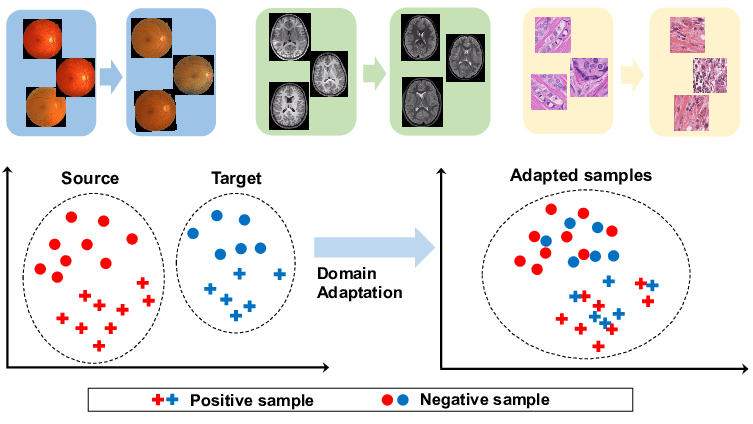
\includegraphics[width=1.0\textwidth]{images/domain_shift_illustration.png}
	\captionof{figure}{Minh họa về Domain Shift. Không gian đặc trưng của miền nguồn (Source) và miền đích (Target) bị lệch nhau. Một bộ phân loại (đường nét đứt) được huấn luyện trên miền nguồn sẽ hoạt động kém trên miền đích.}
	\label{fig:domain_shift_illustration}
\end{center}
% Keyword gợi ý: domain shift machine learning, domain adaptation source target

\subsection{Thích ứng Miền (Domain Adaptation - DA)}
\label{subsec:domain_adaptation}
\textbf{Mục tiêu:} Thích ứng một mô hình đã được huấn luyện trên một miền nguồn có nhiều dữ liệu gán nhãn ($D_S$) để nó hoạt động tốt trên một miền đích ($D_T$) mà chúng ta thường chỉ có dữ liệu không nhãn. Đây là trường hợp phổ biến nhất, được gọi là \textbf{Unsupervised Domain Adaptation (UDA)}.

Ý tưởng cốt lõi của hầu hết các phương pháp DA là cố gắng học một không gian biểu diễn đặc trưng (feature representation space) mà ở đó, sự khác biệt về phân phối giữa miền nguồn và miền đích được giảm thiểu.

\subsubsection{Thích ứng đối nghịch (Adversarial Adaptation)}
\label{subsubsec:adversarial_adaptation}
Lấy cảm hứng từ Mạng Sinh đối nghịch (GAN), phương pháp này sử dụng một trò chơi đối kháng để học các đặc trưng bất biến miền.
\begin{itemize}
	\item \textbf{Kiến trúc:} Hệ thống bao gồm hai thành phần chính:
	\begin{enumerate}
		\item \textbf{Feature Extractor ($G_f$):} Một mạng (ví dụ: CNN) có nhiệm vụ trích xuất đặc trưng từ cả ảnh nguồn và ảnh đích.
		\item \textbf{Domain Discriminator ($G_d$):} Một bộ phân loại nhị phân, được huấn luyện để phân biệt xem một vector đặc trưng đến từ miền nguồn hay miền đích.
	\end{enumerate}
	\item \textbf{Quá trình huấn luyện đối kháng:}
	\begin{itemize}
		\item $G_d$ cố gắng làm tốt nhất công việc của mình: phân biệt các đặc trưng.
		\item $G_f$ cố gắng "đánh lừa" $G_d$ bằng cách tạo ra các đặc trưng cho cả hai miền mà $G_d$ không thể phân biệt được.
	\end{itemize}
	\item \textbf{DANN (Domain-Adversarial Neural Network):} \cite{Ganin2016} là một phương pháp kinh điển, sử dụng một lớp đặc biệt gọi là \textbf{Gradient Reversal Layer (GRL)}. Lớp này hoạt động như một ánh xạ đồng nhất trong quá trình lan truyền xuôi, nhưng lại nhân gradient với một hằng số âm trong quá trình lan truyền ngược. Khi đặt GRL giữa $G_f$ và $G_d$, việc tối thiểu hóa hàm mất mát của $G_d$ sẽ tương đương với việc tối đa hóa nó đối với $G_f$, tạo ra một trò chơi đối kháng minimax trong một kiến trúc duy nhất.
\end{itemize}
Kết quả cuối cùng là $G_f$ học được cách tạo ra các đặc trưng "domain-agnostic", giúp một bộ phân loại được huấn luyện trên các đặc trưng này có thể tổng quát hóa tốt từ miền nguồn sang miền đích.

\subsubsection{Ngẫu nhiên hóa Miền (Domain Randomization)}
\label{subsubsec:domain_randomization}
Thay vì cố gắng làm cho dữ liệu mô phỏng trông giống hệt dữ liệu thực (một nhiệm vụ rất khó), Domain Randomization đi theo một triết lý ngược lại: nếu các biến thể trong môi trường mô phỏng đủ lớn và đa dạng, thì môi trường thực tế sẽ chỉ trông giống như một biến thể khác mà thôi.
\begin{itemize}
	\item \textbf{Cơ chế:} Trong quá trình huấn luyện trên dữ liệu mô phỏng (sim), ngẫu nhiên hóa một cách cực đoan các tham số không liên quan đến tác vụ, chẳng hạn như:
	\begin{itemize}
		\item Vị trí, màu sắc, và cường độ của nguồn sáng.
		\item Kết cấu (texture) của các đối tượng và nền.
		\item Vị trí và góc của camera.
		\item Số lượng và vị trí của các vật thể gây nhiễu.
	\end{itemize}
	\item \textbf{Mục tiêu:} Buộc mô hình phải học các đặc trưng cốt lõi, bất biến của đối tượng, thay vì "overfit" vào các chi tiết bề mặt của môi trường mô phỏng.
	\item \textbf{Ứng dụng:} Đây là kỹ thuật cực kỳ quan trọng và thành công trong lĩnh vực robot, cho phép các mô hình được huấn luyện hoàn toàn trong môi trường ảo có thể được chuyển giao sang robot vật lý (sim-to-real transfer).
\end{itemize}

\begin{center}
	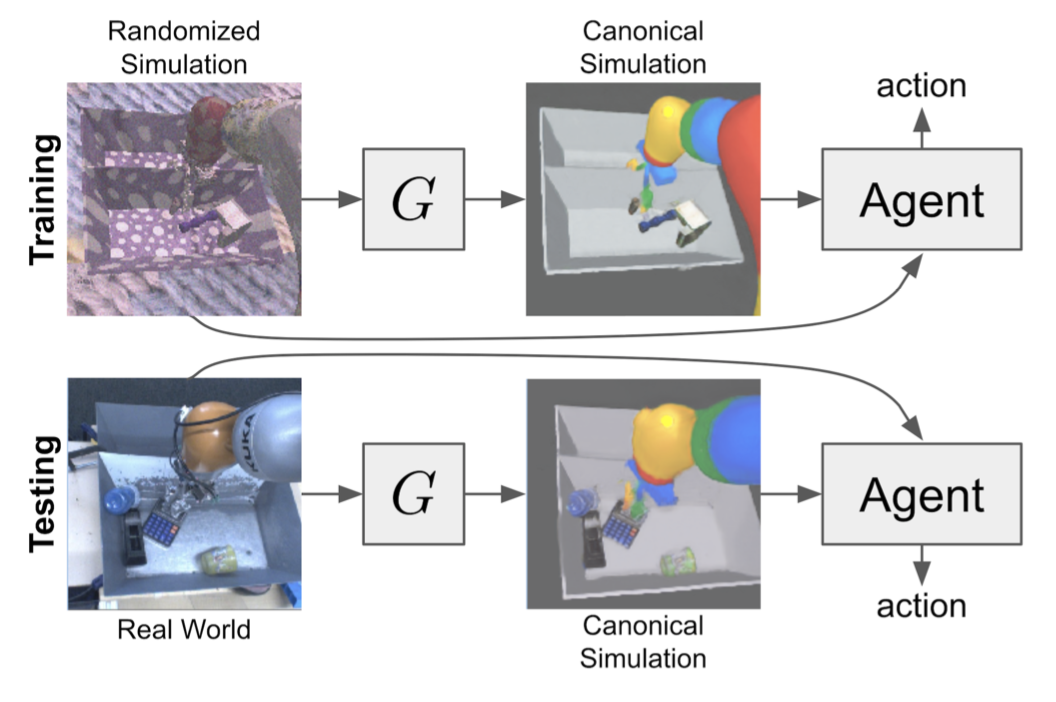
\includegraphics[width=0.9\textwidth]{images/domain_randomization_robotics.png}
	\captionof{figure}{Ví dụ về Domain Randomization. Một cánh tay robot được huấn luyện để nhận dạng và gắp vật thể trong một môi trường mô phỏng với các kết cấu, màu sắc và ánh sáng được ngẫu nhiên hóa một cách cực đoan.}
	\label{fig:domain_randomization}
\end{center}
% Keyword gợi ý: domain randomization robotics, sim-to-real transfer

\subsection{Tổng quát hóa Miền (Domain Generalization - DG)}
\label{subsec:domain_generalization}
\textbf{Sự khác biệt cốt lõi so với DA:} Trong DA, chúng ta có quyền truy cập vào dữ liệu (không nhãn) của miền đích trong quá trình huấn luyện. Trong DG, bài toán khó hơn nhiều: chúng ta được cho dữ liệu từ \textbf{nhiều miền nguồn khác nhau} ($D_{S1}, D_{S2}, ...$) và phải huấn luyện một mô hình duy nhất có khả năng hoạt động tốt trên một \textbf{miền đích hoàn toàn mới và chưa từng thấy} ($D_{T\_unseen}$).

\subsubsection{Các Chiến lược Tổng quát hóa Miền}
\label{subsubsec:dg_strategies}
\begin{description}
	\item[Tăng cường Dữ liệu theo Phong cách Miền:] Sử dụng các kỹ thuật data augmentation nâng cao để mô phỏng sự đa dạng của các miền khác nhau. \textbf{MixStyle} \cite{Zhou2021} là một ví dụ, nó trộn các thống kê đặc trưng (trung bình và độ lệch chuẩn) của các feature map giữa các mẫu từ các miền khác nhau, tạo ra các "phong cách" (styles) mới.
	\item[Học các Biểu diễn Bất biến (Invariant Representation Learning):] Đây là hướng đi chính trong DG, nhằm mục đích tách biệt các đặc trưng "nguyên nhân" (causal features), vốn ổn định qua các miền, khỏi các đặc trưng "giả mạo" (spurious features) chỉ đúng trong một số miền nhất định. \textbf{Invariant Risk Minimization (IRM)} là một khung lý thuyết có ảnh hưởng lớn trong lĩnh vực này.
	\item[Sức mạnh của các Mô hình Nền tảng:] Gần đây, người ta phát hiện ra rằng các mô hình nền tảng như \textbf{CLIP}, được huấn luyện trước trên hàng trăm triệu cặp (ảnh, văn bản) từ internet, tự nhiên có được khả năng tổng quát hóa zero-shot đáng kinh ngạc. Do đã "nhìn thấy" một sự đa dạng khổng lồ về các miền dữ liệu trong quá trình pre-training, các đặc trưng của chúng rất mạnh mẽ và ít bị ảnh hưởng bởi domain shift.
\end{description}

\subsection{Ứng dụng Thực tế}
\label{subsec:da_dg_applications}
Các kỹ thuật DA và DG là cầu nối không thể thiếu để triển khai các hệ thống thị giác trong thế giới thực.
\begin{itemize}
	\item \textbf{Xe tự hành:} Thích ứng các mô hình từ dữ liệu được thu thập vào ban ngày, trời đẹp sang các điều kiện thời tiết xấu (mưa, tuyết, sương mù) hoặc ban đêm.
	\item \textbf{Giám sát bằng Camera:} Một hệ thống nhận dạng người được huấn luyện trên một bộ dữ liệu công khai cần phải được thích ứng để hoạt động với các loại camera khác nhau (góc rộng, hồng ngoại), được lắp đặt ở các độ cao và góc nhìn khác nhau.
	\item \textbf{Chẩn đoán Y tế:} Đảm bảo rằng một mô hình chẩn đoán ung thư từ ảnh chụp X-quang hoạt động ổn định và đáng tin cậy trên các máy chụp từ các nhà sản xuất khác nhau và ở các bệnh viện khác nhau, vốn có các giao thức chụp ảnh và đặc tính nhiễu riêng biệt.
	\item \textbf{Robot Vision:} Cho phép robot được huấn luyện trong thế giới ảo có thể hiểu và tương tác với thế giới vật lý thực, một bài toán được gọi là "sim-to-real gap".
\end{itemize}

\subsection{Kết luận}
Domain Adaptation và Domain Generalization không còn là những chủ đề nghiên cứu mang tính hàn lâm, mà đã trở thành những thành phần thiết yếu trong vòng đời phát triển của các sản phẩm AI thị giác. Chúng giải quyết một trong những vấn đề cơ bản và khó khăn nhất: làm thế nào để xây dựng các mô hình không chỉ hoạt động tốt trên một bộ dữ liệu tĩnh, mà còn có thể thích ứng và duy trì hiệu năng trong một thế giới không ngừng thay đổi. Khi các ứng dụng AI ngày càng trở nên quan trọng và được triển khai ở khắp mọi nơi, tầm quan trọng của việc xây dựng các hệ thống mạnh mẽ và đáng tin cậy trước Domain Shift sẽ chỉ ngày càng tăng lên.

\section*{Tài liệu tham khảo}
\begin{itemize}
	\item[1] Ganin, Y., Ustinova, E., Ajakan, H., Germain, P., Larochelle, H., Laviolette, F., ... \& Lempitsky, V. (2016). Domain-adversarial training of neural networks. \textit{The Journal of Machine Learning Research}, 17(1), 2096-2030. (Paper kinh điển giới thiệu DANN và Gradient Reversal Layer).
	\item[2] Tobin, J., Fong, R., Ray, A., Schneider, J., Zaremba, W., \& Abbeel, P. (2017). Domain randomization for transferring deep neural networks from simulation to the real world. In \textit{2017 IEEE/RSJ International Conference on Intelligent Robots and Systems (IROS)}. (Paper tiên phong về Domain Randomization cho robot).
	\item[3] Zhu, J. Y., Park, T., Isola, P., \& Efros, A. A. (2017). Unpaired image-to-image translation using cycle-consistent adversarial networks. In \textit{Proceedings of the IEEE international conference on computer vision (ICCV)}. (Paper giới thiệu CycleGAN, một công cụ mạnh mẽ để chuyển đổi phong cách miền).
	\item[4] Arjovsky, M., Bottou, L., Gulrajani, I., \& Lopez-Paz, D. (2019). Invariant risk minimization. \textit{arXiv preprint arXiv:1907.02893}. (Giới thiệu khung lý thuyết Invariant Risk Minimization cho Domain Generalization).
	\item[5] Zhou, K., Yang, Y., Qiao, Y., \& Xiang, T. (2021). Domain generalization with robust style normalization. In \textit{Proceedings of the IEEE/CVF conference on computer vision and pattern recognition (CVPR)}. (Giới thiệu MixStyle, một kỹ thuật augmentation hiệu quả cho DG).
	\item[6] Radford, A., Kim, J. W., Hallacy, C., Ramesh, A., Goh, G., Agarwal, S., ... \& Sutskever, I. (2021). Learning transferable visual models from natural language supervision. In \textit{International Conference on Machine Learning (ICML)}. (Paper về CLIP, cho thấy khả năng tổng quát hóa miền vượt trội của các mô hình nền tảng).
\end{itemize}